\part{Implémentation}

\section{Structure du programme}
Nous avons implémenté nos algorithmes en java en utilisant la bibliothèque jgrapht pour la gestion des graphes. Voici la structure générale du programme :\newline

\scalebox{0.7} {
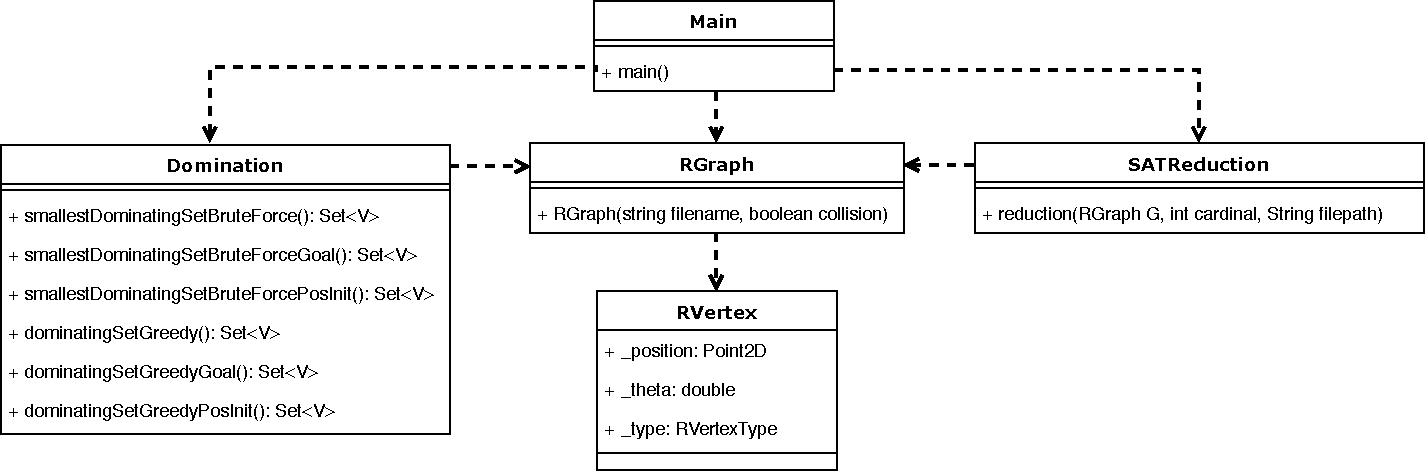
\includegraphics{robotdef.pdf}
} \newline

Le constructeur de la classe RGraph est capable de lire un fichier d'entrée json pour créer un graphe modélisant le problème correspondant. Les sommets de RGraph sont des RVertex. Un RVertex est composé d'une position, d'un angle de tir si le sommet est un sommet de tir et d'un type qui décrit si le sommet est un sommet de tir ou de position (ou un sommet de position surface de réparation dans le cas de l'extension goal). La classe Domination contient les implémentations des algorithmes de résolution et la classe SATReduction la réduction vers SAT. La fonction reduction sauvegarde la formule SAT dans un fichier en format dimacs. Notre programme peut ensuite demander au solveur SAT glucose de tester la satisfaisabilité de cette formule.

\section{Utilisation}

Pour utiliser l'application, compilez tous les fichiers sources dans \textit{robodef/src/main} avec les librairies externes (fichiers .jar) présents dans les dossiers \textit{robotdef/lib\_jgrapht} et \textit{robotdef/lib\_json}.

Lorsque le programme est lancé, vous devez commencer par choisir un fichier au format JSON décrivant le problème dont vous voulez générer une solution (au moins un exemple pour chaque problème est disponible dans le dossier \textit{robotdef/problems}).  Vous devrez ensuite choisir le type de problème (extension) lié au fichier que vous venez de sélectionner.

Le programme utilisera l'algorithme correspondant au type de problème que vous aurez renseigné, sans vérifier la structure du fichier JSON décrivant ce problème. L'utilisation d'un fichier non adapté au problème sélectionné pourrait ne pas donner d'erreur apparente, mais le résultat, s'il en sort un, n'aurait pas de sens.

\subsection{Utilisation de SAT}

L'utilisation de l'algorithme SAT est différent des autres. Pour l'utiliser, il faut tout d'abord aller compiler le code C présent dans \textit{robotdef/glucose-syrup-4.1/simp} avec la commande \textit{make}.

Une fois l'exécutable de glucose généré, vous pouvez lancer notre programme. L'utilisation de SAT ne fonctionne que pour les problèmes normaux (basic problems), il faut donc sélectionner un fichier décrivant un problème de ce type. 

Sélectionnez ensuite SAT comme 


\section{Limitations}

Toutes les extensions n'ont pas été implémentées avec toutes les méthodes. Il n'est pas possible d'utiliser deux extensions en même temps sauf distance minimale qui peut être utilisé en même temps que certaines extensions.

\begin{tabular}{| l | c | c | c | c |}
 \hline		
     & Sans Extension & Plusieurs Buts & Position Initiale & Gardien \\
   \hline 
   Force Brute & 2 & 3 & 4 & 5\\
  \hline  
 Glouton & 2 & 3 & 4  & 5\\
 \hline  
 SAT & 2 & 3 & 4  & 5\\
 \hline  
 Force Brute (Distance Minimale) & 2 & 3 & 4  & 5\\
 \hline  
 Glouton (Distance Minimale) & 2 & 3 & 4  & 5\\
 \hline 
 SAT (Distance Minimale) & 2 & 3 & 4  & 5\\
  \hline  
 \end{tabular}

Nous n'avons pas implémenté le fait de récupérer les positions des défenseurs à partir de la solution renvoyée par glucose. 

\section{Résultats}

La méthode force brute est beaucoup trop lente pour être utilisable lorsque $pos_{step}$ est trop petit (en dessous de $0,4$). \newline

La méthode gloutonne est en revanche très rapide même pour des valeurs de $pos_{step}$ très petites (quelques millisecondes seulement) mais ne donne pas forcément une solution optimale. 
Cependant en pratique la réponse renvoyée par la méthode gloutonne possède généralement le même nombre de défenseurs que la méthode force brute. \newline

La réduction vers SAT permet d'obtenir une solution optimale en un temps beaucoup plus raisonnable. Pour un $pos_{step}$ de $0,2$ la réduction vers SAT prend quelques secondes alors que nous ne savons même pas combien de temps la force brute prendrait pour résoudre ce problème (au moins 30 minutes). Cependant, un temps de réaction de quelques secondes pour une équipe de la robocup serait un désavantage considérable. La méthode gloutonne semble par conséquent plus adaptée.